%% Pour voir les accents de ce fichier, assurez-vous que votre
%% éditeur de texte lise le fichier en utf-8!

%% La classe <dms> est construite au-dessus de <amsbook>, donc
%% <amsmath>, <amsfonts> et <amsthm> sont automatiquement chargés.
%% Pour un mémoire
\documentclass[12pt,twoside,maitrise]{dms}
%% Pour une thèse
%%\documentclass[12pt,twoside,phd]{dms}

\usepackage[utf8]{inputenc} %Obligatoires
\usepackage[T1]{fontenc}    %

%% <lmodern> incorpore les fontes en T1, pour
%% faciliter le dépôt final. Ceci n'est pas la
%% seule option :
%%  1. Si cm-super est installé, vous pouvez enlever <lmodern>
%%     (à ce moment, la police est un peu plus fidèle
%%      au Computer Modern orginal);
%%  2. Si vous avez une police préférée, par exemple,
%%     <times> ou <euler> ou <mathpazo> (et bien d'autres),
%%     alors vous pouvez remplacer <lmodern> ci-bas.
%% Par contre, si vous faîtes face à un problème d'encapsulation
%% lors dépôt final, il se peut que la solution soit d'utiliser <lmodern>.
%% (Parfois le problème est au niveau de l'installation, donc
%%  essayez de compiler sur un autre ordinateur sur lequel vous êtes
%%  certain·e que l'installation est bonne.)
\usepackage{lmodern}

%% Il n'est pas nécessaire d'utiliser <babel>, car
%% les commandes intégrées par la classe <dms>
%% \francais et \anglais font le travail. Néanmoins,
%% certains autres packages nécessitent <babel> (comme
%% <natbib>), donc simplement enlever les % devant <babel>
%% dans ce cas. Attention! Certains packages sont sensibles
%% à l'ordre dans lequel ils sont chargés.
\francais % or
%%\anglais
%%
%%\usepackage[english,frenchb]{babel}

 % ENGLISH OPTION
 % If you call \anglais here before the \begin{document},
 % all the chater's header will be in english, even if you
 % call \francais. To change this, use
 % \entetedynamique

%% La commande \sloppy peut avoir des effets étranges sur les
%% lignes de certains paragraphes.  Dans ce cas, essayez \fussy
%% qui suppresse les effets de \sloppy.
%% (\fussy est normalement le comportement par défaut.)
%% On redéfinit \sloppy, pour tenter de réduire les comportements
%% étranges. Le seul changement apporté à la version originale
%% est la valeur de \tolerance.
\def\sloppy{%
  \tolerance 500%  %9999 dans LaTeX ordinaire, mauvaise idée.
  \emergencystretch 3em%
  \hfuzz .5pt
  \vfuzz\hfuzz}
\sloppy   %appel de \sloppy pour le document
%%\fussy  %ou \fussy

%% Packages utiles.
\usepackage{graphicx,amssymb,subfigure,icomma}
%% icomma       permet d'écrire les nombres décimaux en
%%                  français (p.ex. 1,23 plutôt que 1.23)
%% subfigure    simplifie l'inclusion de figures côtes-à-côtes

%% Packages parfois utiles.
%%\usepackage{dsfont,mathrsfs,color,url,verbatim,booktabs}
%% dsfont       symboles mathématiques \mathds
%% mathrsfs     plus de symboles mathématiques \mathscr
%% color        pour utiliser des couleurs (comparer avec <xcolor>)
%% url          permet l'écriture d'url
%% verbatim     pour écrire du code ou du texte tel quel
%% booktabs     plus de macros pour faire les tableaux
%%                  (voir documentation du package)

%% pour que la largeur de la légende des figures soit = \textwidth
\usepackage[labelfont=bf, width=\linewidth]{caption}

%% les 3 lignes suivante servent à l'affichage de l'index
%% dans le visionneur de pdf. <hyperref> et <bookmark>
%% devraient être les dernier package a être chargé,
%% donc chargez vos packages avant.
\usepackage{hyperref}  % Ajoute les hyperlien
\hypersetup{colorlinks=true,allcolors=black}
\usepackage{hypcap}   % Corrige la position du lien pour les images
\usepackage{bookmark} % Remédie à des petits problème
                      % de <hyperref> (important qu'il
                      % apparaisse APRÈS <hyperref>)

  % Enlever les commentaires du prochaine \hypersetup et
  % le remplir avec l'information pertinente.
  % Ceci ajoute des « méta-données » au pdf.  C'est optionnel,
  % mais recommandé. Vous pouvez voir ces méta-données en
  % ouvrant un visionneur de pdf et en cherchant les propriétés
  % du pdf. (Vous pouvez aussi tapez ' pdfinfo <nom-du-pdf> '
  % dans un terminal.) Ces données sont utiles, par exemple,
  % pour augmenter les chances qu'un algorithme de recherche
  % trouve votre document sur Internet, une fois diffusé.
%%\hypersetup{
%%  pdftitle = {Titre de la thèse / du mémoire},
%%  pdfauthor = {auteur·e},
%%  pdfsubject = {Ex: Transformation de Fourier ; régressions linéaires ; ... },
%%  pdfkeywords = {Ex: mathématiques, statistiques, groupes, variables aléatoires,...}
%%}

%% Définition des environnements utiles pour un mémoire scientifique.
%% La numérotation est laissée à la discrétion de l'auteur·e. L'exemple
%% illustré ici produit « Définition x.y.z »
%%   x = no. chapitre
%%   y = no. section
%%   z = no. définition
%% et la numérotation des corollaires, définitions, etc. se fait
%% successivement.
%%
%% Les macros \<type>name sont telles qu'ils suivent
%% la langue actuelle. (P.ex. si \francais est utilisé,
%% alors \begin{theo} va faire un Théorème et si \anglais
%% est utilisé, \begin{theo} fera un Theorem.)
%%
\newtheorem{cor}{\corollaryname}[section]
\newtheorem{deff}[cor]{\definitionname}
\newtheorem{ex}[cor]{\examplename}
\newtheorem{lem}[cor]{\lemmaname}
\newtheorem{prop}[cor]{Proposition}
\newtheorem{rem}[cor]{\remarkname}
\newtheorem{theo}[cor]{\theoremname}
\theoremstyle{definition}
\newtheorem{algo}[cor]{\algoname}
%% NOTE : Il peut être commode de redéfinir \the<type> pour
%% obtenir la numérotation désirée. Par exemple, pour
%% que les corollaires soit numérotés #section.#sous-section.#sous-sous-section.#paragraphe.#corollaire,
%% on fait
%% \renewcommand\thecor{\theparagraph.\arabic{cor}}

%%%
%%% Si vous préférez que les corollaires, définitions, théorèmes,
%%% etc. soient numérotés séparément, utilisez plutôt un bloc de
%%% commandes de la forme :
%%%

%%\newtheorem{cor}{\corollaryname}[section]
%%\newtheorem{deff}{\definitionname}[section]
%%\newtheorem{ex}{\examplename}[section]
%%\newtheorem{lem}{\lemmaname}[section]
%%\newtheorem{prop}{Proposition}[section]
%%\newtheorem{rem}{\remarkname}[section]
%%\newtheorem{theo}{\theoremname}[section]

%%
%% Numérotation des équations par section
%% et des  tableaux et figures par chapitre.
%% Ceci peut être modifié selon les préférences de l'utilisateur.
\numberwithin{equation}{section}
\numberwithin{table}{chapter}
\numberwithin{figure}{chapter}

%%
%% Si on veut faire un index, il faut décommenter la ligne
%% suivante. Ajouter des mots à l'index avec la commande \index{mot cle} au
%% fur et à mesure dans le texte.  Compiler, puis taper la commande
%% makeindex pour creer les indexs.  Après une nouvelle compilation,
%% vous aurez votre index.
%%

%%\makeindex

%% Il est obligatoire d'écrire à double interligne
%% ou à interligne et demi. On peut soit utiliser
%% le package <setspace> ou \baselinestretch.
%% Le package est un peu plus propre, mais le choix
%% reste à la discrétion de l'usager.
\usepackage[onehalfspacing]{setspace}
 % ou
%%\renewcommand{\baselinestretch}{1.5}

%%%%%%%%%%%%%%%%%%%%%%%%%%%%%%%%%%%%%%%%%%%%%%%%%%%%%%%%%%%%
%%%%%%%%%%%%%%%%%%%%%%%%%%%%%%%%%%%%%%%%%%%%%%%%%%%%%%%%%%%%
%%%%%%%%%%                                     %%%%%%%%%%%%%
%%%%%%%%%% D é b u t    d u    d o c u m e n t %%%%%%%%%%%%%
%%%%%%%%%%                                     %%%%%%%%%%%%%
%%%%%%%%%%%%%%%%%%%%%%%%%%%%%%%%%%%%%%%%%%%%%%%%%%%%%%%%%%%%
%%%%%%%%%%%%%%%%%%%%%%%%%%%%%%%%%%%%%%%%%%%%%%%%%%%%%%%%%%%%
\begin{document}

%%
%% Voici des options pour annoter les différentes versions de votre
%% mémoire. La commande \brouillon imprime, au bas de chacune des pages, la
%% date ainsi que l'heure de la dernière compilation de votre fichier.
%%
%%\brouillon
%%
%%
%% \version est la version de votre manuscrit
%%
\version{1}

%%------------------------------------------------- %
%%              pages i et ii                       %
%%------------------------------------------------- %

%%%
%%% Voici les variables à définir pour les deux premières pages de votre
%%% mémoire.
%%%

\title{Titre du mémoire ou de la thèse}

\author{Nom du candidat}

\copyrightyear{Année de la thèse}

\department{Département de mathématiques et de statistique}

\date{\today} %Date du DÉPÔT INITIAL (ou du 2e dépôt s'il y a corrections majeures)

\sujet{Discipline}
%%\orientation{orientation}%Ce champ est optionnel
%%
%% Voici les disciplines possibles (voir avec votre directeur):
%% \sujet{statistique},
%% \sujet{mathématiques}, \orientation{mathématiques appliquées},
%% \orientation{mathématiques fondamentales}
%% \orientation{mathématiques de l'ingénieur} et
%% \orientation{mathématiques appliquées}

\president{Nom du président du jury}

\directeur{Nom du directeur de recherche}

%%\codirecteur{Nom du 1er codirecteur}         % s'il y a lieu
%%\codirecteurs{Nom du 2e codirecteur}         % s'il y a lieu

\membrejury{Nom du membre de jury}

%%\examinateur{Nom de l'examinateur externe}   %obligatoire pour la these

%% \membresjury{Deuxième membre du jury}  % s'il y a lieu

%%  \plusmembresjury{Troisième membre du jury}    % s'il y a lieu

 % Cette option existe encore, mais elle n'a plus sa place
 % dans la page titre. L'utiliser seulement si le directeur
 % insiste...
%%\repdoyen{Nom du représentant du doyen} %(thèse seulement)

%%
%% Fin des variables à définir. La commande \maketitle créera votre
%% page titre.

\maketitle

 % Pour générer la deuxième page titre, il faut appeler à nouveau \maketitle
 % Cette page est obligatoire.
\maketitle

%%------------------------------------------------- %
%%              pages iii                           %
%%------------------------------------------------- %

\francais

\chapter*{Résumé}

...sommaire et mots clés en français...

%%------------------------------------------------- %
%%              pages iv                            %
%%------------------------------------------------- %

\anglais
\chapter*{Abstract}

...summary and keywords in english...

%%------------------------------------------------- %
%%        page v --- Table de matieres              %
%%------------------------------------------------- %

 % Pour un mémoire en anglais, changer pour
 % \anglais. Noter qu'il faut une permission
 % pour écrire son mémoire en anglais.
%%\anglais
\francais
 % \cleardoublepage termine la page actuel et force TeX
 % a poussé les éléments flottant (fig., tables, etc.) sur
 % la page (normalement TeX les garde en suspend jusqu'à ce
 % qu'il trouve un endroit approprié). Avec l'option <twoside>,
 % la commande s'assure que la prochaine page de texte est sur
 % le recto, pour l'impression. On l'utilise ici
 % pour que TeX sache que la table des matières etc. soit
 % sur la page qui suit.
%% TABLE DES MATIÈRES
\cleardoublepage
\pdfbookmark[chapter]{\contentsname}{toc}  % Crée un bouton sur
                                           % la bar de navigation
\tableofcontents
 % LISTE DES TABLES
\cleardoublepage
\phantomsection  % Crée une section invisible (utile pour les hyperliens)
\listoftables
 % LISTE DES FIGURES
\cleardoublepage
\phantomsection
\listoffigures

%%%%%%%%%%%%%%%%%%%%%%%%%%%%%%%%%%%%%
%% LISTE DES SIGLES ET ABRÉVIATION %
%%%%%%%%%%%%%%%%%%%%%%%%%%%%%%%%%%%%%
%% Il est obligatoire, selon les directives de la FESP,
%% pour une thèse ou un mémoire d'avoir une liste des sigles et
%% des abréviations.  Si vous considérez que de telles listes ne seraient pas
%% pertinentes (si, par exemple, vous n'utilisez aucun sigle ou abré.), son
%% inclusion ou omission est laissé à votre discrétion.  En cas de doute,
%% parlez-en à votre directeur de recherche, le coadministrateur ou au/à la
%% bibliothécaire.
%%
%% Le gabarit inclut un exemple d'une liste « fait à la main ».  Il existe des outils
%% plus sophistiqués si vous devez inclure une multitude de sigles et abréviations.
%% Par exemple, le package <glossaries> peut faire des index élaborés.  Comme
%% son utilisation est technique, il n'y a pas d'exemple directement dans ce gabarit.
%% On invite les gens qui aurait à l'utiliser à lire la documentation officielle,
%% soit en allant sur https://www.ctan.org/, soit en tapant dans un terminal :
%%
%% texdoc glossaries
%%

\chapter*{Liste des sigles et des abréviations}
 % Option de colonnes: definir \colun ou \coldeux
%%% Exemple
%%% \def\colun{\bf} % Première colonne en gras
%%% Pour numéroté les entrées, on peut faire
%%% \newcount\abbrlist
%%% \abbrlist=0
%%% \def\plusun{\global\advance\abbrlist by 1\relax}
%%% \def\colun{\plusun\the\abbrlist. }
%%\def\coldeux{\relax}
\begin{twocolumnlist}{.2\textwidth}{.7\textwidth}
  KQ-Methode & Méthode des moindres carrés, de l'allemand
      \textit{Methode der kleinsten Quadrate}\\
  MCMC  & Monte Carlo par chaînes de Markov, de l'anglais
      \textit{Markov Chain Monte Carlo} \\
  MSE  &  Erreur quadratique moyenne, de l'anglais \textit{Mean Square Error}\\
  NDR & Retract d'un voisinage, de l'anglais \textit{Neighbourhood Deformation Retract}\\
  OLS  &  Moindres carrés ordinaires, de l'anglais \textit{Ordinary Least Square}\\
  ZFC & Théorie des ensembles de Zermelo-Fraenkel avec l'axiome du choix\\
\end{twocolumnlist}
%% L'environnement <threecolumnlist> existe aussi pour trois colonnes.

%%------------------------------------------------- %
%%              pages vi                            %
%%------------------------------------------------- %

\chapter*{Remerciements}

...remerciements...

 %
 % Fin des pages liminaires.  À partir d'ici, les
 % premières pages des chapitres ne doivent pas
 % être numérotées
 %

\NoChapterPageNumber
\cleardoublepage

%%%%%%%%%%%%%%%%%%%%%%%%%%%%%%%%%%%%%%%%%%%%%%%%%%%%%
%%                                                  %
%%   TEXTE DU MÉMOIRE :  introduction page 1,...    %
%%                                                  %
%%%%%%%%%%%%%%%%%%%%%%%%%%%%%%%%%%%%%%%%%%%%%%%%%%%%%

\chapter*{Introduction}

...introduction...

%%------------------------------------------------- %
%%                pages 1                           %
%%------------------------------------------------- %

\chapter{Titre du premier chapitre}

Le 1$^{\text{er}}$ chapitre numéroté. Voici quelques mots en \emph{italique}, en \textbf{gras} et \textsf{sans serif}.

\section{Section un du premier chapitre}

La premi\`ere section du 1$^{\text{er}}$ chapitre.

\subsection {Sous-section un}

Un peu de texte\dots

\subsubsection{Sous-sous-section un}

Encore du texte\dots et un tableau

\begin{table}[htb]
    \centering
    \begin{tabular}{|c||l|c|r|p{0.4\textwidth}|}
        \hline          &          &            &          &                             \\
        \textbf{Option} & g        & c          & d        & \verb|p{0.4\textwidth}|     \\[3mm]
        \hline\hline    &          &            &          &                             \\
        \textbf{Effet}  & À gauche & Au centre  & À droite & Le texte de cette colonne
          est justifié et la largeur de la colonne est fixée à 40\,\% de la zone
          de texte (hors tableau).                                                       \\[3mm]
        \hline
    \end{tabular}
    \caption{Un tableau simple dans le premier chapitre.}
    \label{tab:simple1}
\end{table}
Le tableau \ref{tab:simple1} n'est pas tr\`es garni.

Voici un exemple de pseudo-code. L'exemple utilise
les macros offertent par la classe \texttt{dms}, mais
les utilisateurs peuvent bien utiliser les packages
de leur choix.

\begin{algo} Cet algorithme ne fait rien d'intéressant et
  sert à illustrer un exemple.
 % On aligne les colonnes à l'aide de &
 % et on utilise \cleartabs pour "effacer"
 % l'alignement.
 % Notez qu'il l'alignement est toujours préservé d'un \+
 % à l'autre, c'est pourquoi il est nécessaire d'utiliser
 % \cleartabs lorsque \+ doit oublier l'ancien alignement.
\Hline
\noindent\hbox{\hskip2\parindent\vbox{
\+ \bf Si $n$ \rm est impair, \cleartabs&\bf alors ${\it imprimer}(n)$\rm;\cr
\+     &\bf sinon $n:= n +1$;\cr
\+ \bf Tant que $n < N$~:\cr % Le ~ est un espace insécable
\+ \qquad\cleartabs& \bf ${\it imprimer}(n)$;\cr
\+     &\bf  $n:= n+1$;\cr
\+     &\bf  $j:= j + {\it factoriel}(n)$;\cr
\+ \bf fin;\cr
\+ \bf retourner $j$;\cr
}}
\Hline
\end{algo}

Voici un autre exemple; cette fois le pseudo-code d'une
fonction.

\begin{algo} Cet algorithme inspecte une matrice et
  imprime les entrées impaires et les notes dans un
  tableau qu'il retourne.
\Hline
\noindent\hbox{\kern2\parindent\vbox{
\+ \bf Tableau$^\ast$\ ${\it Imprimer\_Elements\_Impaires}({\bf Matrice}^\ast\ M, {\bf Tableau}^\ast\ T)\ \{$ \cr
\+ \qquad\cleartabs& \bf $m := {\it nb\_ligne}(M)$;\cr
\+     & \bf $n := {\it nb\_col}(M)$;\cr
\+     & \bf Pour $i \in \{1,\ldots, m\}$~:\cr
\+     &\qquad\cleartabs & \bf Pour $j \in \{1,\ldots,n\}$~:\cr
\+     &&\qquad\cleartabs& \bf Si $M(i,j)$ \rm est &impaire, \cr
\+     &&&\hfill&\bf alors~: & \bf ${\it imprimer}(M(i,j))$;\cr
\+     &&&&& \bf $T(i,j) := M(i,j)$;\cr
\+     &&&&\bf fin;&\cr
\+     && \bf fin;\cr
\+     &\bf fin;\cr
\+     &\bf Retourner $T$; &&&& \cleartabs\qquad&\tt\% Un commentaire\cr
\+ \bf $\}$;\cr
}}
\Hline
\end{algo}

\noindent\textbf{Note~:} Les exemples illustrent comment
obtenir un alignement souhaité, mais la mise en page
et le style sont laissés à la discrétion de l'utilisateur.
Autrement dit, {\it l'étudiant ou l'étudiante choisi$\,\cdot$e
ce qui devrait apparaître en italique, en gras, en roman,
en couleur, ce qui doit être indenté. Elle ou il choisit aussi la
langue\/} (mais il est important d'en discuter avec le directeur de recherche
et même de vérifier les règlements en vigueur).

\subsection{Sous-section deux}

Un peu plus de texte\dots

\begin{description}
    \item [exemple] premier element
    \item [second exemple]
\end{description}

\chapter{Quelques exemples}

Voici quelques exemples simples.

\section{Énumérations}

Voici une énumération avec numérotation :
\begin{enumerate}
    \item item 1;
    \item item 2;
    \item item 3.
\end{enumerate}
Maintenant, une énumération sans numérotation avec des marqueurs différents :
\begin{itemize}
    \item Marqueur par défaut;
    \item[$\bullet$] \verb|$\bullet$|;
    \item[$\star$] \verb|$\star$|.
\end{itemize}

\section{Équations mathématiques}

Une équation :
\begin{equation*}
    \otimes^n\,\mathbb{C}^2 \cong \bigoplus_{m=-n/2}^{n/2} W_m.
\end{equation*}

Une autre équation, cette fois-ci numérotée :
\begin{equation}
    \label{eq:eulerlagrange}
    \frac{\partial\mathcal{L}}{\partial\phi^a}-\partial_\mu\frac{\partial\mathcal{L}}{\partial(\partial_\mu\phi^a)}=0,\qquad\mu=0,1,2,3.
\end{equation}
Les équations \eqref{eq:eulerlagrange} précédentes sont appelées \emph{équations d'Euler-Lagrange} ou encore \emph{équations du mouvement}. Dans les calculs suivants,
\begin{align*}
  \delta S
    & = \int_\Omega \mathrm{d}^dx\, \mathcal{L}\left(\phi'^a(x), \partial_\mu\phi'^a(x)\right)
        - \int_\Omega \mathrm{d}^dx\, \mathcal{L}\left(\phi^a(x), \partial_\mu\phi^a(x)\right)\\
    & = \int_\Omega \mathrm{d}^dx\, \left[\delta \phi^a \frac{\partial\mathcal{L}}{\partial\phi^a}
        + \partial_\mu \delta\phi^a \frac{\partial\mathcal{L}}{\partial(\partial_\mu\phi^a)}\right]\\
    & = \int_\Omega \mathrm{d}^dx\, \left[(\delta\phi^a \frac{\partial\mathcal{L}}{\partial\phi^a}
       + \partial_\mu \left(\delta \phi^a \frac{\partial\mathcal{L}}{\partial(\partial_\mu\phi^a)}\right)
       - \delta\phi^a \partial_\mu \frac{\partial\mathcal{L}}{\partial(\partial_\mu\phi^a)}\right]\\
    & = 0,
\end{align*}
aucune ligne n'est numérotée. Alors que dans ce qui suit, la derni\`ere ligne l'est :
\begin{align}
  \delta S
    &= \int_{\Omega'} \mathrm{d}^dx' \,\mathcal{L}\bigl(\phi'^a(x'), \partial'_\mu\phi'^a(x')\bigr)
        - \int_\Omega\mathrm{d}^dx\,\mathcal{L}\bigl(\phi^a(x),\partial_\mu\phi^a(x)\bigr)
        \notag\\
    & = \int_\Omega \mathrm{d}^dx \,\left[\bar{\delta}\phi^a \frac{\partial\mathcal{L}}{\partial\phi^a}
        + \partial_\mu \bar{\delta} \phi^a \frac{\partial\mathcal{L}}{\partial(\partial_\mu\phi^a)}\right]
        + \int_{\partial\Omega}\mathrm{d} \sigma_\mu\,\mathcal{L}
        \bigl(\phi^a,\partial_\mu\phi^a\bigr)\delta x^\mu
        \notag\\
    & = \int_\Omega\mathrm{d}^dx\,\partial_\mu\mathcal{J}^\mu(x).
        \label{eq:variationaction}
\end{align}

\section{Définitions, théorèmes et preuves}

Voici une définition.
\begin{deff}[La définition]
    La définition.
\end{deff}
Voici un théorème.
\begin{theo}[Titre]
    Ceci est vrai !
\end{theo}
\begin{proof}
    Voici la preuve.
\end{proof}
\begin{demo}
    Voici la preuve en gras.
\end{demo}

\section{Construction d'un tableau}

\begin{table}[htb]
    \centering
    \begin{tabular}{|c||l|c|r|p{0.4\textwidth}|}
        \hline            &            &            &            &                                                                                                                            \\
        \textbf{Option}    & g            & c            & d            & \verb|p{0.4\textwidth}|                                                                                                    \\[3mm]
        \hline\hline    &            &            &            &                                                                                                                            \\
        \textbf{Effet}    & À gauche    & Au centre    & À droite    & Le texte de cette colonne est justifié et la largeur de la colonne est fixée à 40\,\% de la zone de texte (hors tableau).    \\[3mm]
        \hline
    \end{tabular}
    \caption{Un tableau simple dans le second chapitre.}
    \label{tab:simple2}
\end{table}
Le tableau \ref{tab:simple2} n'est pas très garni.

\section{Référence à une entrée bibliographique}

La présente section est pour illustrer l'utilisation de
bib\TeX. On cite une référence avec la commande \verb|\cite|.
L'argument est l'étiquette donné à votre référence dans
le fichier \texttt{.bib}, dans notre exemple c'est \texttt{exemple}.
Consulter \cite{exemple} pour \textit{beaucoup} de détail sur \LaTeX.

Ensuite, on compile avec (pdf)\LaTeX\ pour générer un fichier auxilliaire
\texttt{.aux}, on compile bib\TeX\ et on compile \textbf{deux} fois
avec (pdf)\LaTeX.

Les entrées du fichier \verb|.bib| qui ne sont pas référencées
dans le texte ne sont pas ajoutées à la bibliographie.

\section{Insertion de figures}


\begin{figure}[t]
    \centering
    
\includegraphics[width=0.2\textwidth]{figures/cercle.pdf}
    \caption{Un cercle.}
    \label{fig:Cercle}
\end{figure}
La figure \ref{fig:Cercle} est un \emph{cercle}.
\begin{figure}[t]
    \centering
    \subfigure[Un triangle.]{\label{fig:Triangle}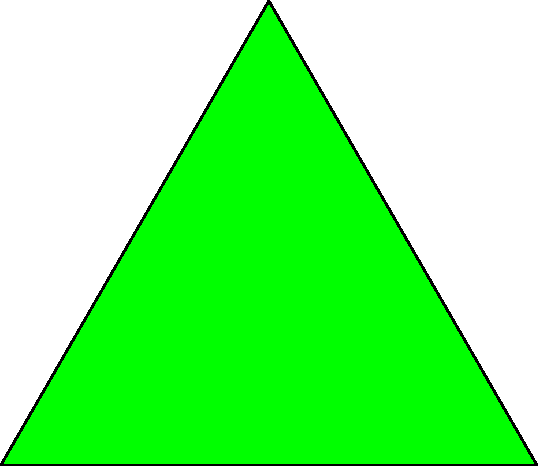
\includegraphics[width=0.2\textwidth]{figures/triangle.pdf}}\hspace{2cm}
    \subfigure[Un carré.]{\label{fig:Carre}
\includegraphics[width=0.2\textwidth]{figures/carre.pdf}}
    \caption{\label{fig:TriCar}Un carré et un triangle.}
\end{figure}
À la figure \ref{fig:TriCar}, le triangle \subref{fig:Triangle} et le carré \subref{fig:Carre} ont été placés côtes-à-côtes grâce à la commande \verb|\subfigure|.

%%--------------%
%%     index    %
%%--------------%

%% S'il y a lieu, décommenter la ligne pour mettre votre index

%%\printindex

%%------------------------------------------------- %
%%         références --- bibliographie             %
%%------------------------------------------------- %
  % Enlever les commentaires de la prochaine commande si vous préférez que le
  % chapitre s'appelle « Références » plutôt que « Bibliographie » (au choix selon le contexte).
%%\let\bibname=\refname

%% Lorsque vous serez prêt à faire afficher votre bibliographie
%% et vos références, enlevez les commandaires des commandes suivantes
%% et donnez le nom de votre fichier .bib à la commande \bibliography{..}
%% (consultez l'exemple au besoin).  Vous pouvez utiliser le style de votre
%% choix.
\bibliographystyle{plain-fr}     % Le style de la bibliographie. Notons que
                                        % les extensions ne sont pas données pour ces deux fichiers.
\def\bibname{R\'ef\'erences bibliographiques} % Nom obligatoire de la section des références.
                                              % On utilise \'e car le é cause des problèmes
                                              % dans la table des matière
%% ENGLISH
 %\def\bibname{References}
\bibliography{ref}     % La base de données contenant des entrées bibliographiques.
                                    % Seules celles référencées dans le texte seront ajoutées
                                    % \`a la bibliographie.

%%------------------------------------------------- %
%%                  Annexe A                        %
%%------------------------------------------------- %

\appendix
\chapter{Le titre}

\section{Section un de l'Annexe A}

...texte...

\chapter{Les différentes parties et leur ordre d'apparition}

J'ajoute ici les différentes parties d'un mémoire ou d'une thèse ainsi
que leur ordre d'apparition tel que décrit dans le guide de
présentation des mémoires et des thèses de la Faculté des études
supérieures.  Pour plus d'information, consultez le guide sur le site
web de la facutlé (www.fes.umontreal.ca).

\newcount\colnum
\colnum=1
\def\i{\number\colnum. \global\advance\colnum by 1\ignorespaces}
\begin{table}[p]
  \begin{center}
    \begin{tabular}{|l|l|r|}\hline
       \noindent\hfil
         \textbf{\strut Ordre des éléments constitutifs du mémoire ou de la thèse}
         \hfil\span\omit\span\omit\\\hline % \span\omit pour couvrir plus d'une
                                           % case sans utiliser le package multirow ou autre
      \i &  La page de titre & obligatoire\\\hline
      \i &  La page d'identification des membres du jury & obligatoire\\\hline
      \i &  Le résumé en français et les mots clés français\kern3em& obligatoires\\\hline
      \i &  Le résumé en anglais et les mots clés anglais & obligatoires\\\hline
      \i &  Le résumé dans une autre langue que l'anglais & obligatoire \\
         &  ou le français (si le document est écrit dans &\\
         &  une autre langue que l'anglais ou le français)&\\\hline
      \i &  Le résumé de vulgarisation& facultatif\\\hline
      \i &  La table des matières, la liste des tableaux,& obligatoires\\
         &   la liste des figures ou autre &\\\hline
      \i &  La liste des sigles et des abréviations& obligatoire\\\hline
      \i &  La dédicace& facultative\\\hline
      \i &  Les remerciements & facultatifs\\\hline
      \i &  L'avant-propos & facultatif\\\hline
      \i &  Le corps de l'ouvrage& obligatoire\\\hline
      \i &  Les index& facultatif\\\hline
      \i &  Les références bibliographiques & obligatoires\\\hline
      \i &  Les annexes & facultatifs\\\hline
      \i &  Les documents spéciaux & facultatifs\\\hline
    \end{tabular}
  \end{center}
\end{table}

\end{document}



\endinput
%%
%% End of file `gabaritmem.tex'.
